\documentclass[12pt,a4paper]{article}

\usepackage[utf8]{inputenc} \usepackage[T1]{fontenc} \usepackage{graphicx}
\usepackage{longtable} \usepackage{tabularx} \usepackage{float}
\usepackage{wrapfig} \usepackage{soul} \usepackage{amssymb}
\usepackage{hyperref} \usepackage{caption} \usepackage{subcaption}
\usepackage{pdfpages} \usepackage{sidecap}


\parindent 0in \usepackage[spanish]{babel}
\setlength{\parskip}{0.5\baselineskip} \usepackage{fullpage}
\usepackage{multirow} \usepackage{multicol} \usepackage{framed}
\usepackage{listings} \usepackage{enumerate}

\usepackage{appendix}


%% DEFINICIONES
\newcommand{\TODO}[1]{{\huge \color{red} \textbf{TODO: }#1 }}
\newcommand{\todo}[1]{{\large \color{red} \textbf{TODO: }#1 }}



\title{Práctica P0}
\author{Luis M. Costero Valero ( lcostero@ucm.es )\\Jesús Doménech
  Arellano ( jdomenec@ucm.es )\\Jennifer Hernández Bécares (
  jennhern@ucm.es )}
\date{}

\begin{document} 
\maketitle

\begin{enumerate}[(a)]
\item \textbf{¿Cuándo la curva es un punto? ¿Contradice esto el teorema fundamental?}\\
  Cuando sus derivadas son 0 para todo punto del intervalo,
  independientemente de su curvatura. Esto no contradice el tma fundamental
  de curvas porque no verifica la hipótesis de estar parametrizada por el
  arco (|c'(s)|=1).

\item \textbf{¿La curva que se obtiene estará siempre parametrizada por la
    longitud de arco? ¿Estará recorrida a velocidad constante? ¿Sabrías
    explicar por qué?}\\
  La curva resultante no estará parametrizada por la longitud de arco, ya
  que para la misma curvatura se pueden obtener distintas curvas en función
  de las condiciones iniciales establecidas. En cambio, la curva sí que
  estará recorrida a velocidad constante, ya que el módulo de la tangente
  no varía a lo largo de la curva.

\item \textbf{Dar un ejemplo de curvatura tal que la curva converja a una
    recta cuando $s \to \infty$ y a una circunferencia cuando $s \to
    -\infty$.}\\
  La curva será una recta cuando la curvatura sea 0, y una circunferencia
  cuando sea un valor constante. Consideramos la siguiente función:
  $$ k(s) = \frac{tan^{-1}(-s^{3})}{\pi}+\frac{1}{2} $$
  tal que verifica que $$\lim_{s\to-\infty}k(s)=1 , \lim_{s \to \infty}
  k(s) = 0$$
  La función $k(s)$ y la curva $c(s)$ vienen representadas por:\\
  
  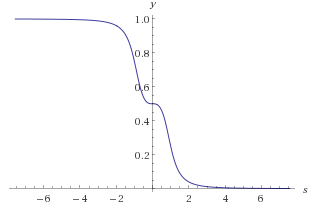
\includegraphics[width=0.4\textwidth]{P0/f.png}\hspace{0.5cm}
  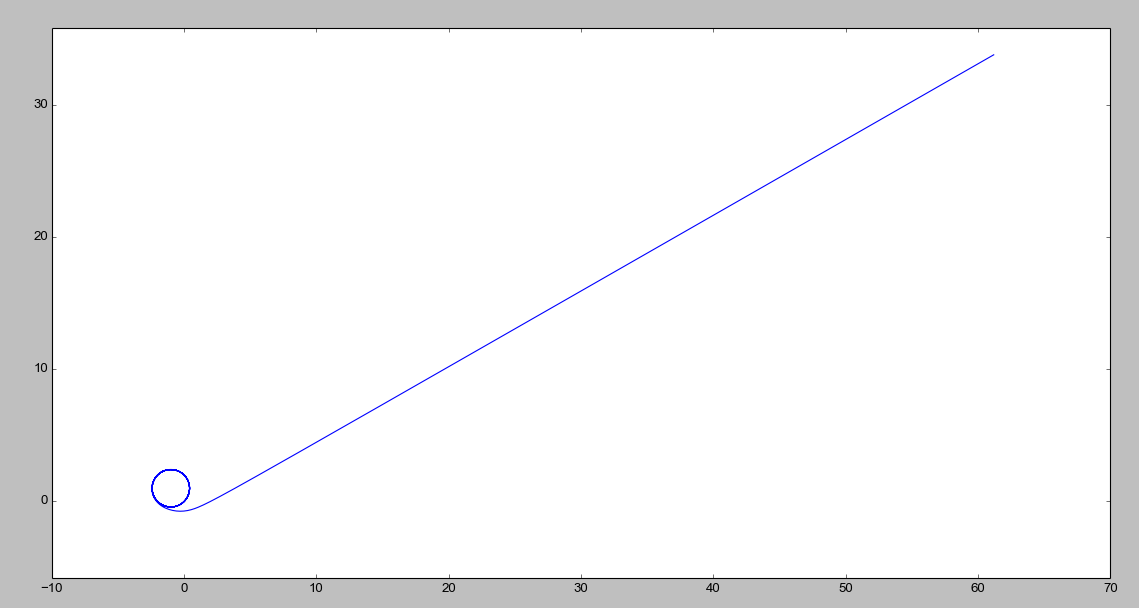
\includegraphics[width=0.5\textwidth]{P0/A.png}
  % \caption{Representación de $k(s)$ a la izquierda y la curva $c(s)$ a la
  % derecha}\,
  
\item \textbf{Dar un ejemplo de curvatura tal que la curva gire siempre
    en sentido antihorario.}\\
  Si la curvatura es positiva, la curva gira en sentido antihorario. Por
  ejemplo, la circunferencia con curvatura $k(s)=1$

\item \textbf{Dar un ejemplo de curvatura periódica, pero tal que la curva
    no sea cerrada}\\
  Si la curvatura está definida por $k(s)=sin(s)$, la curva resultante
  viene representada por la siguiente imagen:\\
  \begin{center}
  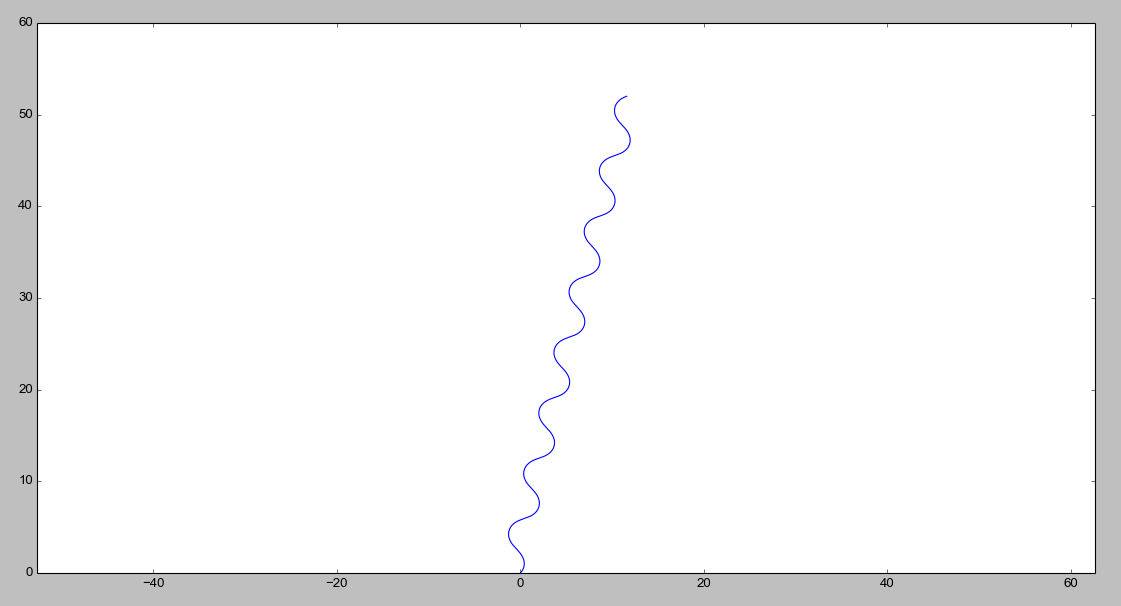
\includegraphics[width=0.7\textwidth]{P0/B.png}
  \end{center}

\item \textbf{Dar un ejemplo de curvatura tal que la curva sea cerrada,
    pero no una circunferencia}\\
  Consideramos una elipse cuya curvatura está definida por:
  $$k(s)=\frac{a*b}{((a*cos(s))^{2}+(b*sin(s))^{2})^{\frac{3}{2}}}$$

\end{enumerate}
\end{document}


